\section{Felicity Distribution and Felicity Factors}
\begin{frame}[t]
\sectionpage\vskip 18pt
\begin{itemize}
    \item<1->	Researchers posited several possible factors that influence rSS felicity:\vskip 18pt
			\begin{itemize}
                \item<1->	{{Degree of World Dissimilarity between ${\color{red}\phi}$ and ${\color{Orange}\psi}$}} \citep{Lewis2017,Krassnig2017}\vskip 18pt
                \item<2->   Contrastive Stress in the second antecedent \citep{Klecha2014a,krassnig2022ReverseSobel}\vskip 9pt
				\item<3->	{Causal links between ${\color{red}\phi}$ and ${\color{Orange}\psi}$} \citep{Klecha2014a}\vskip 9pt
                \item<4->   Counterfactuality of ${\color{red}\phi}$ and ${\color{Orange}\psi}$ \citep{krassnig2022ReverseSobel}\vskip 9pt
				\item<5->	{Epistemic irresponsibility of considering ${\color{red}\phi}$ without ${\color{Orange}\psi}$} \citep{Moss2012}
			\end{itemize}
\end{itemize}
\end{frame}

\subsection{Dynamic World Orderings and Relevance}
\begin{frame}[t]
\subsectionpage\vskip 9pt%
\begin{itemize}
    \item \citet{Lewis2017} proposed the following factor:\vskip 9pt
        \begin{itemize}
            \item<2-> rSS with dissimilar antecedent world sets are felicitous
            \item<3-> rSS with similar antecedent world sets are infelicitous
        \end{itemize}
\end{itemize}\vskip 18pt
\visible<4->{
\begin{minipage}[h]{0.55\linewidth}
\begin{table}[h]
    \begin{tabular}{l||c|c}
                &   Dissimilar     &   Similar\\\hline\hline
          SS    &   \checkmark  &   \checkmark\\
          rSS   &   \checkmark  &   \#
    \end{tabular}
\end{table}
\end{minipage}}\vskip 9pt
\begin{itemize}
    \item<5-> Tough to verify via informal native speaker judgements
    \item<6-> No experimental work on rSS so far\vskip 9pt
    \item<7-> So, we conducted an experiment to test \citepos{Lewis2017} predictions
\end{itemize}
    
\end{frame}

\subsubsection{Experiment}
\begin{frame}<3->[t]
\subsectionpage
	
	\textbf{Empirical Testing of \citet{Lewis2017}}\vskip 9pt
    \begin{itemize}
        \item<3-> Participants (n=41 after excl.) were asked to rate target items on a scale from 1 to 5\vskip 9pt
            \begin{itemize}
                \item<4-> 1 = Sounds very natural
                \item<4-> 5 = Sounds very unnatural
            \end{itemize}\vskip 9pt
        \item<5-> Four target conditions
            \begin{itemize}
                \item<6-> Control (SS \& other felicitous conditional sequences)
                \item<7-> Similar (non-counterfactual rSS where ${\color{red}\phi}\land{\color{Orange}\psi}$ and $\color{red}\phi$ are similar by context)
                \item<7-> Dissimilar (non-counterfactual rSS where ${\color{red}\phi}\land{\color{Orange}\psi}$ and $\color{red}\phi$ are dissimilar by context)
                \item<8-> Disjoint (rSS where ${\color{red}\phi}\land{\color{Orange}\psi}$ was counterfactual%
                )
            \end{itemize}\vskip 9pt
        \item<9-> All items were acausal by nature and indicated contrastive stress
    \end{itemize}
\end{frame}

\begin{frame}[t]
    \subsectionpage\visible<3->{
    \begin{minipage}{0.425\linewidth}
    \begin{figure}[ht!]
    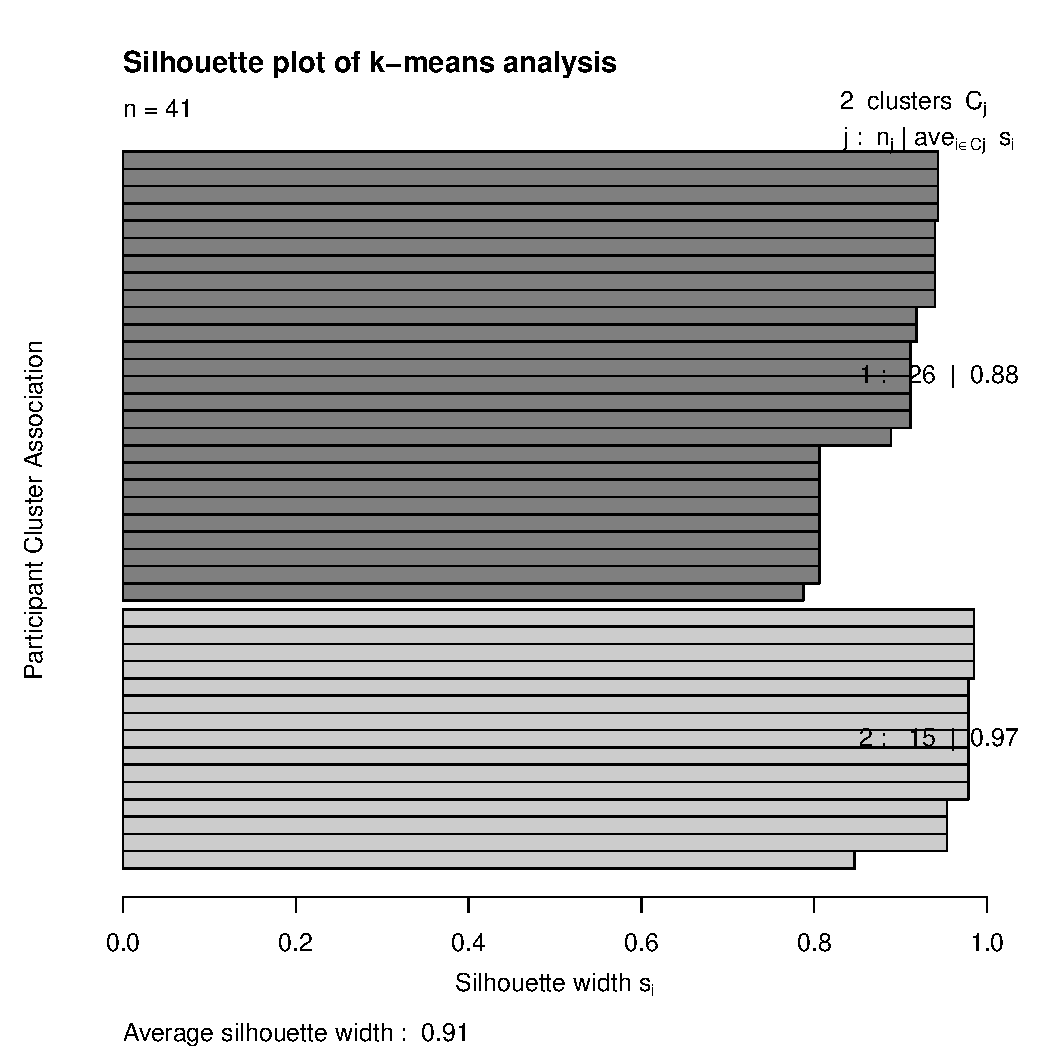
\includegraphics[width=\linewidth,page=1,trim=0pt 30pt 0pt 30pt]{graphics/silhouette.pdf}
\end{figure}
\end{minipage}}%
\begin{minipage}[t]{0.575\linewidth}\vspace*{-40mm}
    \begin{itemize}
        \item<1-> Dissimilar condition results seemed polarising\vskip 9pt
        \item<2-> Conducted a k-means analysis on results\vskip 9pt
        \item<4-> Two clusters with very high average confidence
    \end{itemize}
\end{minipage}
\end{frame}

\begin{frame}[t]
    \subsectionpage\vskip 7.5pt
    \hspace*{45mm}\textbf{Cluster 1}\hspace{72.5mm}\textbf{Cluster 2}\vspace{-7.5mm}
    \begin{figure}[ht!]
\begin{minipage}{0.9\linewidth}
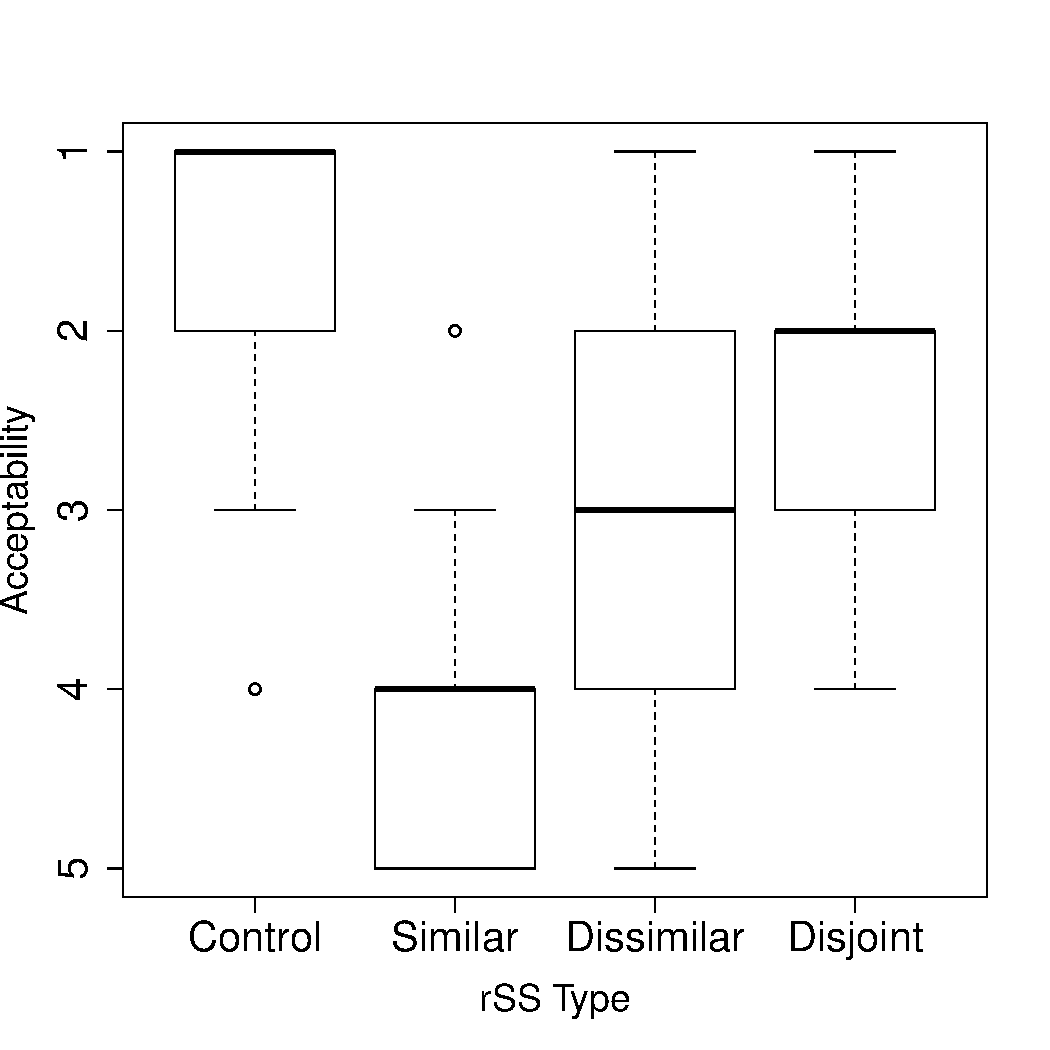
\includegraphics[width=0.425\linewidth,page=1]{graphics/boxplots.pdf}\hspace{10mm}
\includegraphics[width=0.425\linewidth,page=2]{graphics/boxplots.pdf}
\end{minipage}%
\end{figure}
\end{frame}

\begin{frame}[t]
\subsectionpage\vskip 9pt
\begin{itemize}
    \item<1-> No significant difference between clusters except dissimilar rSS condition\vskip 9pt
        \begin{itemize}
            \item<1-> First cluster: Acceptability judgements go haywire\vskip 9pt
        \end{itemize}
    \item<1-> Both clusters: Counterfactual/Disjoint condition almost perfect\vskip 9pt
    \item<1-> Second cluster: No significant difference between dissimilar and similar condition\vskip 18pt
    \item<2-> We therefore reject \citepos{Lewis2017} hypothesis\vskip 9pt
    \item<3-> Dissimilarity does not reliably increase the odds of felicity
\end{itemize}
\end{frame}

\begin{frame}[t]
\subsectionpage\vskip 9pt
\begin{itemize}
    \item<1->	Researchers posited several possible factors that influence rSS felicity:\vskip 18pt
			\begin{itemize}
                \item<1->	{\sout{Degree of World Dissimilarity between ${\color{red}\phi}$ and ${\color{Orange}\psi}$}} \citep{Lewis2017,Krassnig2017}\vskip 18pt
                \item<1->   Contrastive Stress in the second antecedent \citep{Klecha2014a,krassnig2022ReverseSobel}\vskip 9pt
				\item<1->	{Causal links between ${\color{red}\phi}$ and ${\color{Orange}\psi}$} \citep{Klecha2014a}\vskip 9pt
                \item<1->   Counterfactuality of ${\color{red}\phi}$ and ${\color{Orange}\psi}$ \citep{krassnig2022ReverseSobel}\vskip 9pt
				\item<1->	{Epistemic irresponsibility of considering ${\color{red}\phi}$ without ${\color{Orange}\psi}$} \citep{Moss2012}
			\end{itemize}
\end{itemize}
\end{frame}

\subsection{Contrastive Stress}
\begin{frame}[t]
    \subsectionpage\vskip 9pt
    \begin{itemize}
        \item<1-> \citet{Klecha2014a}: Some overtly different lexical item must be contrastively stressed\vskip 9pt
        \item<2-> \citet{krassnig2022ReverseSobel}: Auxiliary verbs may be contrastively stressed instead\vskip 9pt
        \item<3-> Without any kind of contrastive stress, rSS are infelicitous
    \end{itemize}\vskip 9pt
    \visible<4->{
    	\ex.[\ref{ex:match}]	 \label{ex:contrastaux-good}\textit{(Holding up a dry match, with no water around)} If {\color{red}I had struck this match} and {\color{Orange}it had been soaked}, {\color{OliveGreen}it would} not {\color{OliveGreen}have lit}. But if {\color{red}I \MakeUppercase{had} struck this match}, {\color{OliveGreen}it would have lit}.
    
    }
    \visible<5->{
    	\ex.\label{ex:contrastaux-bad}\textit{(Holding up a dry match, with no water around)} If {\color{red}I had struck this match} and {\color{Orange}it had been soaked}, {\color{OliveGreen}it would} not {\color{OliveGreen}have lit}. \#But if {\color{red}I{'d} struck this match}, {\color{OliveGreen}it would have lit}.
    
    }\vskip 9pt
    \begin{itemize}
        \item<6-> We take the presence of contrastive stress for granted for all future factors
    \end{itemize}
\end{frame}

\subsection{Causality}
\begin{frame}[t]
    \subsectionpage\vskip 9pt
    \begin{itemize}
        \item<1-> \citet{Klecha2014a}: another factor is causality\vskip 9pt
            \begin{itemize}
                \item<2-> If ${\color{red}\phi}$ precedes ${\color{Orange}\psi}$ on some causal chain, then the rSS is infelicitous
            \end{itemize}\vskip 18pt
        \item<3-> \textbf{Acausal rSS}~~~($\color{red}\phi$ does not causally precede $\color{Orange}\psi$)
        \end{itemize}
 \visible<4->{
    	\ex.[\ref{ex:match}]	 \label{ex:acausaloki}\textit{(Holding up a dry match, with no water around)} If {\color{red}I had struck this match} and {\color{Orange}it had been soaked}, {\color{OliveGreen}it would} not {\color{OliveGreen}have lit}. But if {\color{red}I \MakeUppercase{had} struck this match}, {\color{OliveGreen}it would have lit}.%
    
    }
    \vskip 18pt
    \begin{itemize}
        \item<5-> \textbf{Causal rSS}~~~($\color{red}\phi$ causally precedes $\color{Orange}\psi$)
    \end{itemize}
    \visible<6->{
    \ex.\label{ex:causalnoki}\textit{(Holding up a dry match, with no water around)} If {\color{red}I had struck this match} and {\color{Orange}it had snapped}, {\color{OliveGreen}it would} not {\color{OliveGreen}have lit}. \#But if {\color{red}I \MakeUppercase{had} struck this match}, {\color{OliveGreen}it would have lit}.
    
    }
\end{frame}

\subsection{Counterfactuality}
\begin{frame}[t]
    \subsectionpage\vskip 9pt
    \begin{itemize}
        \item<1-> \citet{krassnig2022ReverseSobel}: Non-Counterfactuality has exact same impact as causality\vskip 9pt
            \begin{itemize}
                \item<2-> If $\color{red}\phi$ and ${\color{Orange}\psi}$ are non-counterfactual, then the rSS is infelicitous
            \end{itemize}\vskip 18pt
        \item<3-> \textbf{Counterfactual Acausal rSS}~~~($\color{red}\phi$ and $\color{Orange}\psi$ are counterfactual)
        \end{itemize}
    \visible<4->{
    	\ex.[\ref{ex:match}]	 \label{ex:rss-cf-good}\textit{(Holding up a dry match, with no water around)} If {\color{red}I had struck this match} and {\color{Orange}it had been soaked}, {\color{OliveGreen}it would} not {\color{OliveGreen}have lit}. But if {\color{red}I \MakeUppercase{had} struck this match}, {\color{OliveGreen}it would have lit}.
    
    }\vskip 18pt
    \begin{itemize}
        \item<5-> \textbf{Non-Counterfactual Acausal rSS}~~~($\color{red}\phi$ and $\color{Orange}\psi$ are non-counterfactual)
    \end{itemize}
    \visible<6->{
    	\ex.\label{ex:rss-ncf-bad}\textit{(Holding up a dry match)} If {\color{red}I struck this match tomorrow} and {\color{Orange}it was soaked}, {\color{OliveGreen}it would} not {\color{OliveGreen} light}. \#But if {\color{red}I \MakeUppercase{were} to strike this match tomorrow}, {\color{OliveGreen}it would light}.
    
    }
\end{frame}

\subsection{Epistemic Dismissal}
\begin{frame}[t]
    \subsectionpage
    \begin{itemize}
        \item<1-> \citet{Moss2012}: If {\color{Orange}$\psi$} is (responsibly) epistemically dismissed, the rSS is felicitous\vskip 6pt
        \item<2-> \citet{krassnig2022ReverseSobel}: Epistemic dismissal of {\color{Orange}$\psi$} rescues any contrastively stressed rSS\vskip 14pt
        \item<3-> \textbf{Epistemically Undismissed Non-Counterfactual Causal rSS}~~~($\color{Orange}\psi$ is undismissed)
    \end{itemize}
    \visible<4->{
    	\ex.\label{ex:rss-no-exclusion}\textit{(Holding up a dry match)} If {\color{red}I struck this match tomorrow} and {\color{Orange}it snapped}, {\color{OliveGreen}it would} not {\color{OliveGreen} light}. \#But if {\color{red}I \MakeUppercase{were} to strike this match tomorrow}, {\color{OliveGreen}it would light}.
    
    }\vskip 14pt
    \begin{itemize}
        \item<5-> \textbf{Epistemically Dismissed Non-Counterfactual Causal rSS}~~~($\color{Orange}\psi$ is dismissed)
    \end{itemize}
    \visible<6->{
    	\ex.\label{ex:rss-exclusion}\textit{(Holding up a dry match)} If {\color{red}I struck this match tomorrow} and {\color{Orange}it snapped}, {\color{OliveGreen}it would} not {\color{OliveGreen} light}. But we all know that I'm the national champion at match striking and never snap a match. So, if {\color{red}I \MakeUppercase{were} to strike this match tomorrow}, {\color{OliveGreen}it would light}.
    
    }
\end{frame}

\begin{frame}[t]
    \subsectionpage
    \begin{itemize}
        \item<1-> This dismissal may also be covert via context\vskip 18pt
        \item<2-> \textbf{Epistemically Dismissed Non-Counterfactual Causal rSS}~~~($\color{Orange}\psi$ is dismissed)
    \end{itemize}
    \visible<2->{
    	\ex.\label{ex:rss-exclusion-covert}\textit{(The speaker knows that Mary would never agree to marry John, which is unbeknownst to the other discourse participant.)} Well, let me put it like this: If {\color{red}John proposed to Mary tomorrow} and {\color{Orange}she said yes}, {\color{OliveGreen}he would be very happy}. But if {\color{red}John \MakeUppercase{were} to propose to Mary tomorrow}, {\color{OliveGreen}he would} not {\color{OliveGreen} be happy at all}.
    
    }
\end{frame}

\subsection*{Summary}
\begin{frame}[t]
\subsectionpage\vskip 9pt
\begin{itemize}
    \item<1-> Contrastive stress allows for rSS felicity\vskip 9pt
    \item<2-> Causality and Non-Counterfactuality render rSS infelicitous\vskip 9pt
    \item<3-> Epistemic dismissal of {\color{Orange}$\psi$} rescues all contrastively stressed rSS
\end{itemize}\vskip 18pt
\visible<4->{
\begin{minipage}[h]{0.9\linewidth}
\begin{table}[h]
\caption{Felicity distribution, presupposing the presence of contrastive stress}\vskip -18pt
\resizebox{\textwidth}{!}{%
    \begin{tabular}{l||c|c|c|c|c|c|c}
                &   \multicolumn{3}{|c|}{Acausal}     &  \multicolumn{3}{|c}{Causal}\\\hline
                & CF  &   \multicolumn{2}{|c|}{Non-CF}    & \multicolumn{2}{|c|}{CF}  &   \multicolumn{2}{|c}{Non-CF}\\\hline
                &   & Undismissed & Dismissed   &  Undismissed & Dismissed & Undismissed & Dismissed\\\hline\hline
          SS    &   \checkmark  &   \checkmark  &   N/A  &   \checkmark    &   N/A  &   \checkmark & N/A\\
          rSS   &   \checkmark\ref{ex:match}  &   \#\ref{ex:rss-ncf-bad}  &   \checkmark  &   \#\ref{ex:causalnoki}  & \checkmark &   \#\ref{ex:rss-no-exclusion}    &   \checkmark\ref{ex:rss-exclusion}
    \end{tabular}}
\end{table}
\end{minipage}}
    
\end{frame}
